\section{Theorie}

\subsection{Bragg-Streuung}

\subsection{Detektion der Neutronen}

genutzte Quellen: \cite{PRuD, He3_vacutec, Knoll_2010, Herforth_Koch_1986}


\subsubsection{Zählrohrcharakteristik}

Zur Detektion von ionisierender Strahlung werden oft Zählrohre verwendet. Es existieren Ionisationskammern,  Proportional-  und Geiger-Müller-Zählrohre. Sie folgen alle einem ähnlichen Aufbau, arbeiten jedoch bei unterschiedlichen Spannungen.  Dies kann an der Zählrohrcharakteristik verdeutlicht werden. Sie zeigt die Abhängigkeit der Anzahl der gemessenen Impulse von der  Zählrohrspannung. Zu sehen sind verschiedene Bereiche:

%\begin {figure} [!htb] = zwinge auf exakte Position

\begin{figure} [!htb]
	
\includegraphics [width=10cm] {pics/Kennlinie_Zaehlrohr.png}
	\centering
	\caption {Zählrohrcharakteristik\protect\footnotemark }
\end{figure}
\footnotetext {Bild aus: \url{https://upload.wikimedia.org/wikipedia/commons/thumb/d/d3/Kennlinie_Zaehlrohr-GER.svg/720px-Kennlinie_Zaehlrohr-GER.svg.png}  [06.06.2018 21:31 Uhr]}

\begin{description}
	\item[Bereich I: Rekombination] Die Spannung zwischen Kathode und Anode ist so gering, dass ein Teil der Elektronen auf dem Weg zur Anode mit den Ionen im Zählgas rekombinieren. Oft ist es hier nicht einmal möglich, eine Messung durchzuführen.  

	\item[Bereich II: Sättigungsbereich] Die Spannung ist groß genug, sodass alle durch die Strahlung direkt erzeugten Elektronen (Primärelektronen) die Anode erreichen. In diesem Spannungsbereich werden Ionisationskammern betrieben. Anhand der erreichten Impulshöhe/Ladungsmenge lassen sich Rückschlüsse auf die Art und Energie der eingetroffenen Teilchen schließen. 
	
	\item[Bereich III: Proportionalbereich] Wird die Spannung weiter erhöht, wird es den beschleunigten Primärelektronen möglich, weitere Gasmoleküle durch Zusammenstoß zu ionisieren (Stoßionisation), wodurch sogenannte Sekundärelektronen entstehen. Dies ist möglich, wenn die kinetische Energie der Elektronen größer als die Ionisationsenergie der neutralen Zählgasatome wird. Die stattfindende Sekundärionisation ist in diesem Bereich proportional zur primären Ionisation. Dadurch ist es auch hier möglich, Rückschlüsse auf Art und Energie der einfallenden Teilchen zu ziehen. In diesem Bereich werden Proportionalzählerrohre wie der in diesem Experiment verwendete He3-Detektor betrieben.
	
	\item [Bereich IV: Auslösch- oder Plateaubereich] Durch weitere Erhöhung der Spannung erreicht man einen Bereich, in dem die Sekundärionisation Lawinencharakter annimmt. Während es im Bereich III nur den energiereicheren Elektronen möglich war, Sekundärelektronen zu erzeugen, produziert nun jedes Primärelektron produziert hierbei eine Lawine von Sekundärelektronen. Daher erhöht sich die Anzahl der gezählten Impulse nicht mehr merklich, wenn die Spannung weiter steigt, da alle einfallenden Teilchen detektiert werden. Es ist nur noch eine reine Zählung möglich, Art und Energie der einfallenden Teilchen können nicht mehr bestimmt werden. In diesem Spannungsbereich werden Geiger-Müller-Zählrohre betrieben. 
	\item [Bereich V: Dauerentladung]
\end{description}

\subsubsection{Funktionsweise des $^3He$ Detektor}
\begin{wrapfigure} {R} {10 cm}
	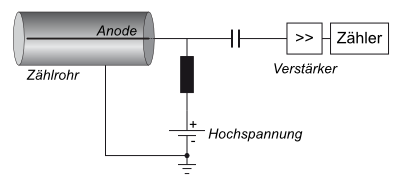
\includegraphics {pics/schematic_construction_counting_tube.png}
	\caption {Schematischer Aufbau eines Proportionalzählrohrs\protect\footnotemark}
\end{wrapfigure}
\footnotetext {Bild aus: \url{https://lp.uni-goettingen.de/get/image/4795}  [18.06.2018 00:06 Uhr]}

Zur Messung der gestreuten Neutronen im vorliegenden Experiment wird ein Helium3 ($^3He$)- Detektor verwendet. Bei Neutronen handelt es sich um ungeladene Teilchen. Um sie nachweisen zu können, müssen aus ihnen erst durch Wechselwirkung mit Materie geladene Teilchen erzeugt werden, die sich mithilfe eines elektrischen Feldes beschleunigen und schließlich messen lassen. Daher besteht ein Detektor für Neutronen immer aus einem Targetmaterial und dem eigentlichen Detektor. Die Targetmoleküle müssen bestimmte Eigenschaften erfüllen. Sie sollten einen möglichst hohen Wirkungsquerschnitt für die stattfindende Kernreaktion der Neutronen besitzen, das genutzte Isotop sollte eine hohe Isotopenhäufigkeit haben oder sich einfach anreichern lassen. Zudem sollte der Q-Wert (kinetische Energie nach der Reaktion, die aus der Bindungsenergie des zerfallenen Nukleons stammt) der Reaktion möglichst groß sein, um möglichst große Energien der Reaktionsprodukte zu erhalten, die sich gut von den Ereignissen verursacht durch Gamma-Strahlung unterscheiden lassen (dazu später mehr). Im vorliegenden Detektor wird He3 sowohl als Target- als auch als Detektormaterial verwendet. Es findet folgende Kernreaktion mit den Neutronen statt (Neutronenenergien unter 20 MeV): 
\ce{n + ^3He -> p + ^3H + 764 keV}, 
Der Detektor selbst arbeitet als Proportionalzählrohr. Dies besteht aus einem metallischen, zylindrischen Rohr und einem auf der Zylinderachse befindlichen Metalldraht. Zwischen dem Rohr (Kathode) und dem Metalldraht (Anode) wird eine Spannung angelegt, sodass ein elektrisches Feld im Inneren des Rohrs entsteht. Das Rohr selbst ist mit einem Zählgas gefüllt, in diesem Fall mit Helium-3. Die Neutronen wechselwirken mit dem Helium wie oben beschrieben und erzeugen ein Proton und einen Tritiumkern (Triton). Diese geladenen Teilchen sind nun in der Lage, Gasatome zu ionisieren. Dadurch werden Elektronen frei, die zur Anode wandern. Die Arbeitsspannung des elektrischen Feldes ist entsprechend so gewählt, dass einige Elektronen kurz vor der Anode in der Lage sind, weitere Gasatome zu ionisieren, wodurch Sekundärelektronen entstehen. Die Elektronen, die die Anode erreichen, erzeugen dort einen Strompuls, der über einen Widerstand in eine Spannung umgewandelt wird, die dann elektronisch weiterverarbeitet und gezählt werden kann. Die Erzeugung von Sekundärelektronen führt zu einer Verstärkung des Messsignals, der sogenannte Gasverstärkungsfaktor ist ein Maß für diese Verstärkung. Er ist als Proportionalitätsfaktor zwischen der im Gesamten erzeugten Ladung Q und den diese Ladung erzeugenden, ursprünglichen, geladenen Teilchen $n_0$ definiert: 
\begin{equation*}
Q = n_0 e M
\end{equation*}
Im Arbeitsbereich des Proportionalzählrohrs ist er konstant, da der Bereich, indem eine für die Gasmultiplikation nötige Feldstärke herrscht, auf einen sehr engen Raum um die Anode beschränkt (klein im Vergleich zum gesamten Gasvolumen im Detektor) ist. Die erzeugten Elektronen bewegen sich zunächst zur Anode, ohne weitere Atome zu ionisieren. Daher durchläuft jedes Teilchen unabhängig von seiner Anfangsposition den gleiche Multiplikationsprozess. Deshalb ist der generierte Spannungspuls proportional zur primären Ionisation durch das einfallende Teilchen.

\subsubsection{Wirkungsquerschnitt der stattfindenden Kernreaktion und Effizienz des $^3He$ Detektors}
Die Effizienz des Detektors berechnet sich nach näherungsweise nach folgender Formel:

\begin{equation}
	\epsilon = 1-e^{-\sum_{a} (E) L}
\end{equation}

$ \sum_{a} (E) $ = makroskopischer Wirkungsquerschnitt der Absorption von $^3He$ in Abhängigkeit von der Neutronenenergie E \\ %erzwungener Zeilenumbruch
L = aktive Länge des Zählrohrs

Der Wirkungsquerschnitt des $^3He$ für die Absorption von Neutronen ist in Abbildung \ref{crosssection_He_3} zu sehen. Er hängt maßgeblich von der Neutronenenergie ab und ist mit Ausnahme hoher Neutronenenergien proportional zu $\frac{1}{\nu}$. Für thermische Neutronen mit einer mittleren Energie von 0,039 eV beträgt er 5330 barn und ist damit wesentlich höher als der Wirkungsquerschnitt anderer zur Neutronendetektion genutzter Zählgase wie $^6Li$ oder $^{10}B$, was auch den wesentlichen Vorteil der Verwendung des $^3He$ als Zählgas für die Neutronendetektion darstellt. 
 
\begin{figure} [!htb]
	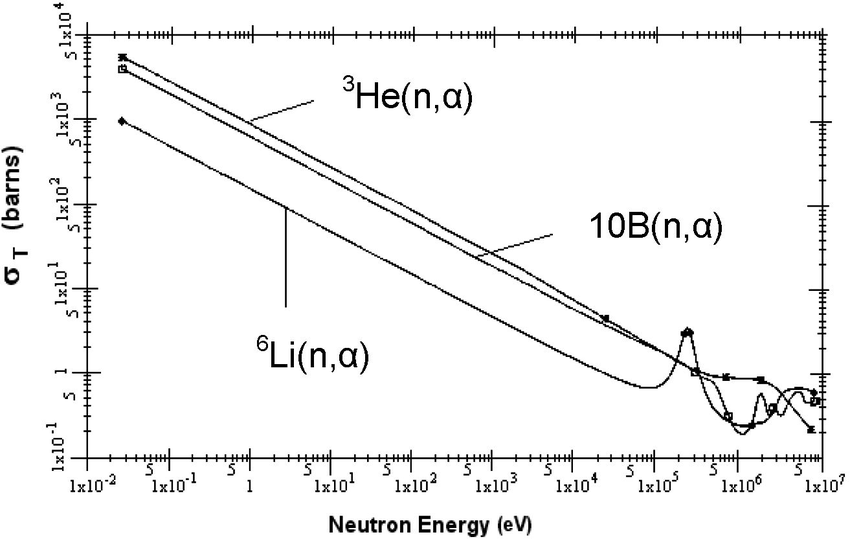
\includegraphics [width=10cm] {pics/cross_section_He3_B10_Li_6.png}
	\centering
	\caption {Wirkungsquerschnitt von $^3He$ im Vergleich mit $^6Li$ und $^{10}B$ \protect\footnotemark }
	\label{crosssection_He_3}
\end{figure}
\footnotetext {Bild aus: \url{https://www.researchgate.net/profile/Ghiraldo_Murillo/publication/262699256/figure/fig1/AS:392502357053440@1470591262568/3-Hen-p-10-Bn-a-and-6-Lin-a-cross-sections-as-a-function-of-incident-neutron.ppm}  [17.06.2018 18:46 Uhr]}

\subsubsection{Bestimmung der Arbeitsspannung des $^3He$ Detektors}
Für eine exakte Messung mittels des He3-Detektors muss eine günstige Arbeitsspannung gefunden werden. Sie muss so gewählt werden, dass jedes ionisierende Teilchen genau eine Stoßentladung hervorruft, damit die Proportionalität zur Energie der einfallenden Strahlung erhalten bleibt. 
Aus der oben beschriebenen Zählrohrcharakteristik lässt sich die Charakteristik eines Proportionalzählrohres schon erahnen. Nicht gut zu erkennen ist, dass sich auch im Bereich des Proportionalzählrohres ein Plateau ausbildet. In Abbildung \ref{charakteristik} ist die Charakteristik eines Proportionalzählrohrs dargestellt. Die Ausbildung des Plateaus bedeutet, dass jedes einfallende Teilchen detektiert wird. Die genaue Lage des Plateaus hängt von vielen Faktoren wie der Form des Zählrohrs, dem verwendeten Gas und dessen Partialdruck oder wie in der Abbildung ersichtlich von der Größe des Diskriminatorlevels ab. Auch wird die Länge und der Anstieg vor dem Plateau durch verschiedene Faktoren wie das Diskriminatorlevel oder die Divergenz der eintreffenden Strahlung beeinflusst. Die Charakteristik des Detektors kann durch Zählratenmessungen bei verschiedenen angelegten Detektorspannungen bestimmt werden. Die Arbeitsspannung wird schließlich so gewählt, dass sie im ersten Drittel des Plateaus liegt, um eine möglichst große Entfernung vom Auslöschbereich zu gewährleisten, da hier die gewünschte Proportionalität zwischen Zählrate und Energie der einfallenden Strahlung nicht mehr gilt. Für den im Experiment verwendeten Detektor wurde so eine Arbeitsspannung von 1100 V festgelegt.  

\begin{figure} [!htb]
	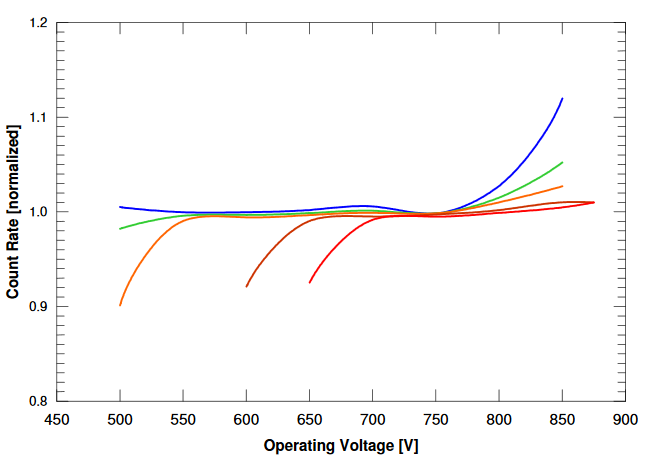
\includegraphics [width=10cm] {pics/characteristic_proportional_counter.png}
	\centering
	\caption {Charakteristik des Proportionalzählrohrs bei unterschiedlichen Diskriminatorleveln \protect\footnotemark }
	\label{charakteristik}
\end{figure}
\footnotetext {Bild aus: \cite{He3_vacutec}}

\subsubsection{Probleme und Messunsicherheiten des $^3He$ Detektors}




%\begin{itemize}
%	\item Brennstoffabbrand,
%	\item Vergiftung des Brennstoffs oder
%	\item Temperatureffekte
%\end{itemize}




